\documentclass{article}
\usepackage{tikz}
\usetikzlibrary{shapes.geometric, arrows}

\tikzstyle{startstop} = [rectangle, rounded corners, minimum width=3cm, minimum height=1cm,text centered, draw=black, fill=red!30]
\tikzstyle{process} = [rectangle, minimum width=3cm, minimum height=1cm, text centered, draw=black, fill=blue!30]
\tikzstyle{decision} = [diamond, minimum width=3cm, minimum height=1cm, text centered, draw=black, fill=green!30]
\tikzstyle{arrow} = [thick,->,>=stealth]

\begin{document}

% diagrama de la funcion principal
\section*{Sistema A: Función Principal}
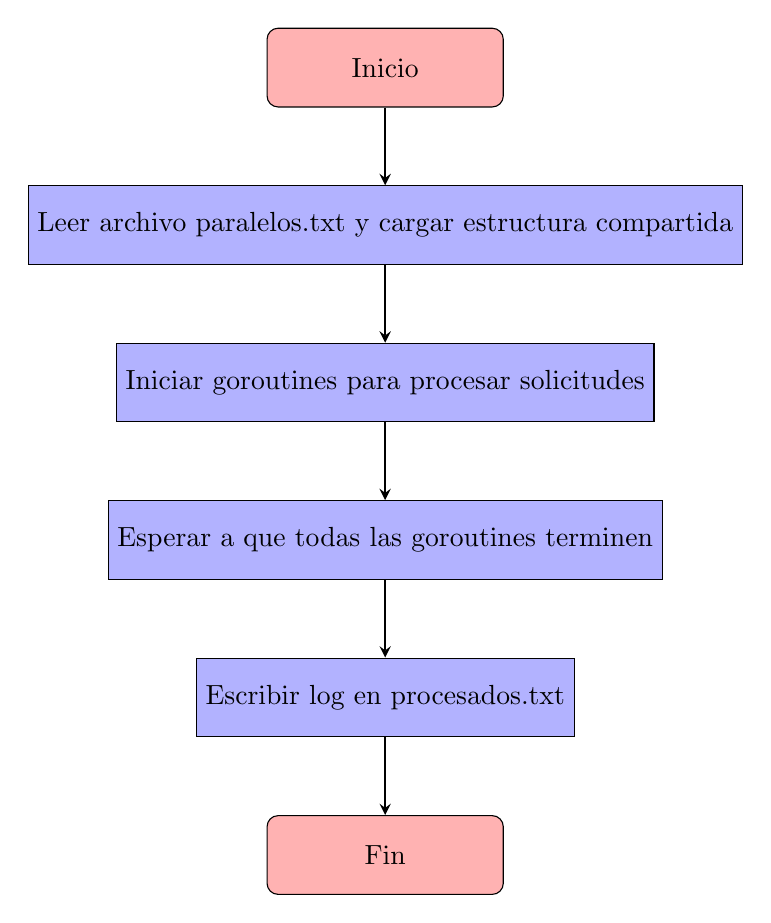
\begin{tikzpicture}[node distance=2cm]

\node (start) [startstop] {Inicio};
\node (readParalelos) [process, below of=start] {Leer archivo paralelos.txt y cargar estructura compartida};
\node (goroutines) [process, below of=readParalelos] {Iniciar goroutines para procesar solicitudes};
\node (wait) [process, below of=goroutines] {Esperar a que todas las goroutines terminen};
\node (log) [process, below of=wait] {Escribir log en procesados.txt};
\node (end) [startstop, below of=log] {Fin};

\draw [arrow] (start) -- (readParalelos);
\draw [arrow] (readParalelos) -- (goroutines);
\draw [arrow] (goroutines) -- (wait);
\draw [arrow] (wait) -- (log);
\draw [arrow] (log) -- (end);

\end{tikzpicture}

\newpage 

% diagrama de goroutines
\section*{Sistema A: Goroutines}
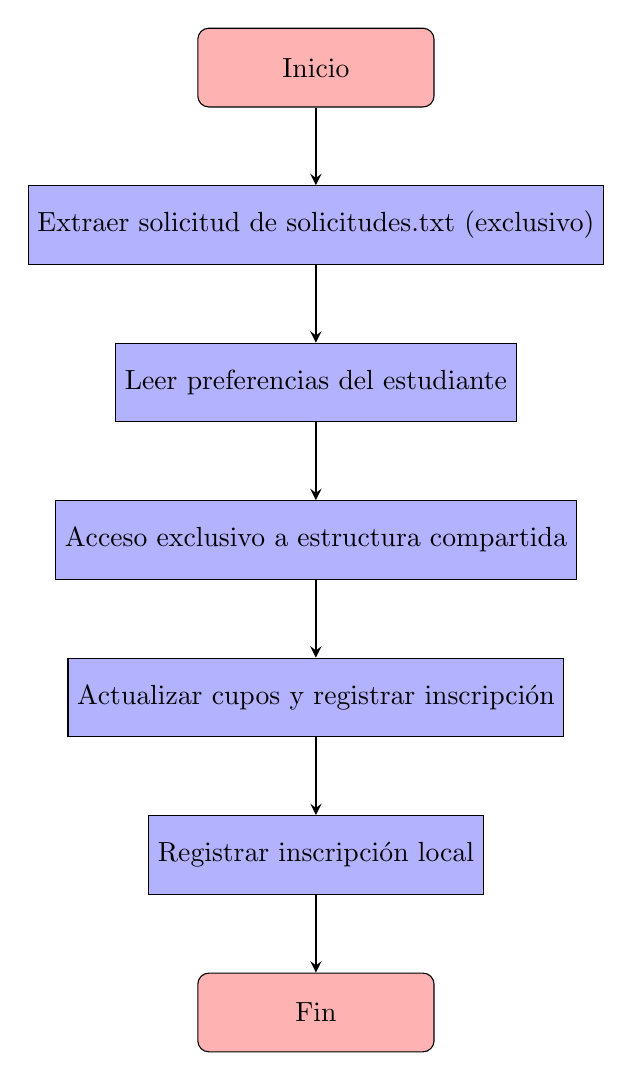
\begin{tikzpicture}[node distance=2cm]

\node (startG) [startstop] {Inicio};
\node (readRequest) [process, below of=startG] {Extraer solicitud de solicitudes.txt (exclusivo)};
\node (readPreferences) [process, below of=readRequest] {Leer preferencias del estudiante};
\node (accessShared) [process, below of=readPreferences] {Acceso exclusivo a estructura compartida};
\node (update) [process, below of=accessShared] {Actualizar cupos y registrar inscripción};
\node (logG) [process, below of=update] {Registrar inscripción local};
\node (endG) [startstop, below of=logG] {Fin};

\draw [arrow] (startG) -- (readRequest);
\draw [arrow] (readRequest) -- (readPreferences);
\draw [arrow] (readPreferences) -- (accessShared);
\draw [arrow] (accessShared) -- (update);
\draw [arrow] (update) -- (logG);
\draw [arrow] (logG) -- (endG);

\end{tikzpicture}

\end{document}
